\pdfminorversion=4 % bug with acroread 
\documentclass[10pt]{beamer}

%% beamer template and options 
\mode<presentation>
{
  \usetheme{CambridgeUS}
  \usefonttheme{serif}
  \useoutertheme{default}
}\setbeamertemplate{navigation symbols}{} 



\usepackage[utf8]{inputenc}
\usepackage{xcolor,comment,cancel}
\specialcomment{extended}{}{}    
\excludecomment{extended}
\usepackage{../styles/authordate1-4-beamer}

\usepackage{pgfplots}
\usepackage{xspace}
\usepackage{amsmath}
\usepackage{wasysym}
\usepackage{tikz}
\usetikzlibrary{automata}
\usetikzlibrary{arrows}
\usetikzlibrary{shapes}
\usetikzlibrary{snakes}
\usetikzlibrary{arrows.meta,intersections}
\tikzstyle{every picture}+=[remember picture]
\usetikzlibrary{decorations.markings}






\title[IDL@BME-BIN] % (optional, use only with long paper titles)
{Introduction to Deep Learning} 
\subtitle{Machine Learning basics}

\author[A. Allauzen] % (optional, use only with lots of authors)
{Alexandre Allauzen}



\institute[ESPCI/Dauphine/PSL] % (optional, but mostly needed)
{
\includegraphics[height=3em]{../logos/espci_blue.png}\hfill
\raisebox{1.75ex}{\includegraphics[height=1.5em]{../logos/dauphine.png}}\\
\hfill\includegraphics[height=3em]{../logos/logomiles_white.pdf}
}




\date{12 and 13/10/2020} % (optional)





\DeclareMathOperator*{\argmax}{argmax}
\DeclareMathOperator*{\argmin}{argmin}

\newcommand{\ngram}{\mbox{$n$-gram}\xspace} 



%% important : red + bf 
\def\important#1{{\bf \color{red} #1\/}}


%%% basics : 
\newcommand{\real}{\ensuremath{\mathbb{R}}}
\newcommand{\vct}[1]{\ensuremath{\mathbf{#1}}} % a vector / matrix is in bold
\newcommand{\seq}[1]{\ensuremath{\boldsymbol{#1}}}

\newcommand{\transp}[1]{\ensuremath{{#1}^{t} }} % transposition 
%\newcommand{\scal}[2]{\left\langle #1 , #2 \right\rangle} % scalair
%product
\newcommand{\scal}[2]{#1^t#2} % scalair product
\newcommand{\mydot}[2]{\ensuremath{ \transp{#1} #2}} % dot prod
\newcommand{\norm}[1]{\ensuremath{|| #1 ||}} % l2
\newcommand{\normabs}[1]{\ensuremath{ || #1 ||_{1} }} % l1




% vertical vector 
\newcommand{\vv}[1]{
	\left(
	\begin{array}[c]{c}
		#1 
	\end{array}
	\right)
}
% backeted vertical vector 
\newcommand{\vvb}[1]{
	\left[
	\begin{array}[c]{c}
		#1 
	\end{array}
	\right]
}
% raw vertical vector 
\newcommand{\vvr}[1]{
	\begin{array}[c]{c}
		#1 
	\end{array}
}





% words sequences sentences 
\newcommand{\ws}{{w}} % 
\newcommand{\wseq}{{\mathbf{\ws}}} % 
\newcommand{\length}{{L}} % 
\newcommand{\wsseq}[2]{{\ws_{#1}^{#2}}} % word subsequence
\newcommand{\word}[1]{{\it #1}} % an example
\newcommand{\vocab}{{\mathcal{V}}} % vocab

\newcommand{\asymb}{\ensuremath{a}} % symbol of *one* element of the
                                % alignment sequence
\newcommand{\ssymb}{\ensuremath{s}} % symbol of *one* element of the source
\newcommand{\tsymb}{\ensuremath{t}} % symbol of *one* element of the target


\newcommand{\aseq}{\ensuremath{\mathbf{\asymb}}} % alignment sentence
\newcommand{\sseq}{\ensuremath{\mathbf{\ssymb}}} % source sentence
\newcommand{\tseq}{\ensuremath{\mathbf{\tsymb}}} % target sentence


% misc 
\newcommand{\BigO}[1]{\ensuremath{\operatorname{O}\bigl(#1\bigr)}}
\newcommand{\bos}{\texttt{\textless s\textgreater}} 
\newcommand{\eos}{\texttt{\textless/s\textgreater}} 


% machine learning i/o and parameters ...
% params for model 
\newcommand{\param}{\ensuremath{\theta}} 
\newcommand{\params}{\ensuremath{\boldsymbol{\theta}}}
\newcommand{\nfeats}{\ensuremath{D}} % 

\newcommand{\x}{\ensuremath{\seq{x}}} % 
\newcommand{\X}{\ensuremath{\seq{X}}} % 
\newcommand{\y}{\ensuremath{\seq{y}}} % 
\newcommand{\z}{\ensuremath{\seq{z}}} % 
\newcommand{\w}{\ensuremath{\seq{w}}} % 
\newcommand{\pa}{\ensuremath{\seq{a}}} % 
\newcommand{\pb}{\ensuremath{\seq{b}}} % 

\newcommand{\W}{\seq{W}}
\newcommand{\V}{\seq{V}}
\newcommand{\pgrad}[1]{\nabla_{#1}}
\newcommand{\vgrad}[2]{\ensuremath{\nabla_{#1} #2}}

%%%%%%% data and loss
\newcommand{\nsamples}{\ensuremath{N}}
\newcommand{\ploss}{\ensuremath{l}} % for one datapoint
\newcommand{\class}{\ensuremath{{c}}} %
\newcommand{\rvclass}{\ensuremath{{C}}} %  the class as a RV 
\newcommand{\sid}[1]{\ensuremath{_{(#1)}}} % sample id
\newcommand{\tid}[1]{_{(#1)}} % time index for parameters
\newcommand{\exi}{\ensuremath{\x\sid{i}}} % 
\newcommand{\classi}{\ensuremath{\class\sid{i}}} % 
\newcommand{\nclasses}{\ensuremath{C}} % 
\newcommand{\yi}{y\sid{i}}  % prediction for sample i 

\newcommand{\dataset}{\ensuremath{\mathcal{D}}} % training data
\newcommand{\datax}{\ensuremath{\mathcal{X}}} % training data, x part
\newcommand{\datay}{\ensuremath{\tilde{\mathcal{Y}}}} % training data y part  
\newcommand{\datac}{\ensuremath{\tilde{\mathcal{C}}}} % training data c part (classes)
\newcommand{\ty}{\ensuremath{\tilde{y}}} % the supervised answer
\newcommand{\fullloss}{\ensuremath{\mathcal{L}(\params;\dataset)}}

%%% 
\newcommand{\nlaw}{\mathcal{N}}
\newcommand{\bern}{\ensuremath{\pi}}



%%%%%%%%%%%%%%%%%%%%%%%%%%%%%%%%%%%%%%%%%%%%%%%%%%%%%%%%%%%%
% a vector as a grid 
% 1: x 
% 2: y
% 3: the number of cells 
% The template :
% \node[rectangle,rounded corners,  draw, fill=red!20, text width=0.3*\textwidth, minimum height=6ex]  (label) at (0,0) {Hello} ;
\newcommand{\xvector}[3]{%
  \draw[step=.25] (#1-0.001,#2) grid (#1+0.25,#2+#3*0.25 );%
}


%%%%%%%%% macro et redefinition 
\AtBeginSection[]
{
  \begin{frame}<beamer>
    \frametitle{Outline}
    \tableofcontents[currentsection]
  \end{frame}
}


\begin{document}
\tikzset{->-/.style={decoration={
  markings,
  mark=at position .5 with {\arrow{>}}},postaction={decorate}}}

\begin{frame}
  \titlepage
\end{frame}

  \begin{frame}<beamer>
    \frametitle{Outline}
    \tableofcontents
  \end{frame}
 


%%%%%%%%%%%%%%%%%%%%%%%%%%%%%%%%%%%%%%%%%%%%%%%%%%%%%%%%%%%%%%%%%%%%%%%%
  % General information :
  % websites, drive
  % labs / courses
  % eval. 
  
  
%%% 
% Course introduction
% Machine Learning : overview
% Learn from data: an output from an input, a decision, a representation, ...
% The main tasks in ML 
% Deep learning and feature ing.
% Roadmap
\section{Introduction}
%%%%%%%%%%%%%%%%%%%%%%%%%%%%%%%%%%%%%%%%%%%%%%%%%%%%%%%%%%%%%%%
% Course introduction
% Machine Learning : overview
% Learn from data: an output from an input, a decision, a representation, ...
% The main tasks in ML 
% Deep learning and feature ing.
%%%%%%%%%%%%%%%%%%%%%%%%%%%%%%%%%%%%%%%%%%%%%%%%%%%%%%%%%%%%%%%
\begin{frame}{Starter: a ``simple'' question}
  \framesubtitle{What it is ?}
    \begin{columns}
      \column{0.3\textwidth} %%%%%%%%%%%%%%%%%
      \begin{center}
        \includegraphics[width=\textwidth]{../figs/dog_drawing}
        \\[3ex]\pause
        \includegraphics[width=\textwidth]{../figs/dog-sad}\pause
      \end{center}
      \column{0.6\textwidth} %%%%%%%%%%%%%%%%%

      \begin{block}{Can you write an algorithm to answer ?}
        \pause
        \begin{itemize}
        \item What is the input space ? 
        \item What do you want to predict ? \\  human generated ? resolution ? 
          real ? outdoor ? the type of dogs ?
        \item The output space ? (binary, multi-class, regression)
        \end{itemize}
      \end{block}
      \begin{block}{And then ?}
        \pause
        \begin{itemize}
        \item What are the features ? 
        \item The decision rule ? 
        \item The evaluation criterion ? 
        \end{itemize}
      \end{block}
    \end{columns}
  \end{frame}

  
%%%%%%%%%%%%%%%%%%%%%%%%%%%%%%%%%%%%%%%%%%%%%%%%%%%%%%%%%%%%%%%
\begin{frame}{Starter: a less ``simple'' question}
    \begin{columns}
      \column{0.3\textwidth} %%%%%%%%%%%%%%%%%
      \begin{center}
        \includegraphics[width=\textwidth]{../figs/object_detection}
      \end{center}
      \column{0.6\textwidth} %%%%%%%%%%%%%%%%%
      \begin{block}{Can you write an algorithm to answer ? }
        \begin{itemize}
        \item What is the input space ? 
        \item What do you want to predict ? \\  a set of tagged bounding boxes
        \item The output space ?\\ multi-class depending on the application
        \end{itemize}
      \end{block}
      \begin{block}{And then ?}
      \pause
      \begin{itemize}
      \item Two tasks: segmentation and classification (joint)
      \item What are the features ? 
      \item The decision rule ?
      \item The evaluation criterion ? 
      \end{itemize}
    \end{block}
    \end{columns}
  \end{frame}

%%%%%%%%%%%%%%%%%%%%%%%%%%%%%%%%%%%%%%%%%%%%%%%%%%%%%%%%%%%%%%%
\begin{frame}{Starter: a less ``simple'' question}
  \framesubtitle{Named Entity Recognition (NER)}
  \begin{columns}
      \column{0.65\textwidth} %%%%%%%%%%%%%%%%%
      \begin{center}
        \includegraphics[width=\textwidth]{../figs/ner}
      \end{center}
      \column{0.35\textwidth} %%%%%%%%%%%%%%%%%
      Can you write an algorithm ?
      % Just gather list of NE but it is not enough
      % language is ambiguous (e.g. Tim Cook)
      % language is evolving (new TV star, new places, new language of interest, ...)
      % answer is obvious (most of the time), but hard to explain
      \begin{itemize}
      \item The input space ? 
      \item The prediction ? \\  %tagged text segments 
      \item The output space ?\\ %multi-class depending on the application
      \end{itemize}
    \end{columns}\pause
    \begin{block}{Just build lists of Named entities ?} 
      \begin{itemize}
      \item language is ambiguous (e.g. Tim Cook, 1984, ... )
      \item language is evolving with new ``people'', places, domain specific terms, ...
      \item answer is obvious (most of the time), but hard to explain
     \end{itemize}
  \end{block}
\end{frame}


%%%%%%%%%%%%%%%%%%%%%%%%%%%%%%%%%%%%%%%%%%%%%%%%%%%%%%%%%%%%%%%
\begin{frame}{The Machine Learning way}
\framesubtitle{How to make a ‘computer’ do a specific task?}
\begin{block}{Traditional approach (old AI)}
A program is:
\begin{itemize}
\item hand-coded
\item specific set of instructions to complete the task
\item can be explained and proved, ``always'' gives the correct answer
\end{itemize}
\end{block}


% The inductive bias (also known as learning bias) of a learning
% algorithm is the set of assumptions that the learner uses to predict
% outputs given inputs that it has not encountered.[1]

% In machine learning, one aims to construct algorithms that are able
% to learn to predict a certain target output. To achieve this, the
% learning algorithm is presented some training examples that
% demonstrate the intended relation of input and output values. Then
% the learner is supposed to approximate the correct output, even for
% examples that have not been shown during training. Without any
% additional assumptions, this problem cannot be solved exactly since
% unseen situations might have an arbitrary output value. The kind of
% necessary assumptions about the nature of the target function are
% subsumed in the phrase inductive bias.

% A classical example of an inductive bias is Occam's razor, assuming
% that the simplest consistent hypothesis about the target function is
% actually the best. Here consistent means that the hypothesis of the
% learner yields correct outputs for all of the examples that have
% been given to the algorithm.
\begin{block}{Machine Learning}
A program is:
\begin{itemize}
\item trained or learnt 
\item from large amount of annotated data 
\item algorithm + inductive bias
\item it works ... on average
\end{itemize}
\end{block}
\end{frame}



\begin{frame}{Machine learning: the main tasks}
  \framesubtitle{Supervised classification}
  \begin{center}
    \tikz[baseline=0]{ \node at (-2,0)
      {\includegraphics[height=0.25\textheight]{figs/mnist_5.pdf}}; %
      \node at (-0.4,0) {:}; \xvector{0}{-0.75}{6} }
    $\x \in \real^{784} \ \longrightarrow \class  \in\{0, 1,2, \ldots ,9
    \}$
  \end{center}
  \begin{itemize}
  \item $\dataset= (\exi , \classi )_{i=1}^{\nsamples}$ 
  \item \important{Supervised} learning of a \important{classification} task
  \end{itemize}
\end{frame}

\begin{frame}{Machine learning: the main tasks}
  \framesubtitle{Supervised binary classification}
  \begin{center}
    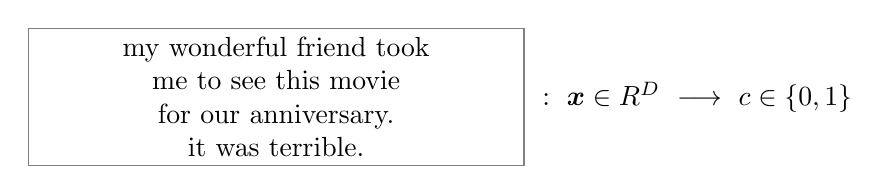
\begin{tikzpicture}
        %%%%%%%%%%%%%%%%%%%%%
      \node[anchor=east,draw=gray,text width=0.5\textwidth,align=center] (review) at
      (0,0) {my wonderful friend took me to see this movie \\for our
        anniversary. \\ it was terrible.};
      %%%%%%%%%%%%%%%%%%%%%
      \node[anchor=west] (txt) at (0.1,0) {$: \ \x \in \real^{\nfeats} \ \longrightarrow \ \class \in\{0, 1\}$};
    \end{tikzpicture}
  \end{center}

  \begin{itemize}
  \item $\dataset= (\exi , \classi )_{i=1}^{\nsamples}$ 
  \item Supervised learning of a \important{binary} classification task
  \end{itemize}

\end{frame}


\begin{frame}{Machine learning: the main tasks}
  \framesubtitle{Supervised regression}
  \begin{center}
    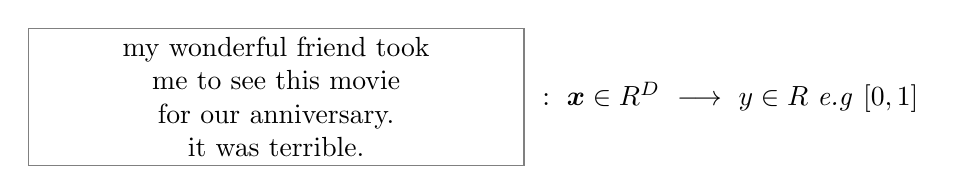
\begin{tikzpicture}
      %%%%%%%%%%%%%%%%%%%%% 
      \node[anchor=east,draw=gray,text width=0.5\textwidth,align=center] (review) at
      (0,0) {my wonderful friend took me to see this movie \\for our
        anniversary. \\ it was terrible.};
      %%%%%%%%%%%%%%%%%%%%%
      \node[anchor=west] (txt) at (0.1,0) {$: \ \x \in \real^{\nfeats}
        \ \longrightarrow \ y \in \real$ \textit{e.g} $[0, 1]$ };
    \end{tikzpicture}
  \end{center}

  \begin{itemize}
  \item $\dataset= (\exi, {\y}\sid{i})_{i=1}^{\nsamples}$ 
  \item Supervised learning of a \important{regression} task
  \end{itemize}
\end{frame}



\begin{frame}{Machine learning: the main tasks}
  \framesubtitle{Unsupervised learning / Clustering}
  \begin{columns}
    \column{0.45\textwidth}
    \begin{figure}[htb]
      \centerline{
%        \includegraphics[height = 0.6\textheight]{book_pile}
        \scalebox{0.15}{\includegraphics{../figs/book_pile}}
      }
    \end{figure}
    \column{0.1\textwidth}
    \begin{Huge}
    $\Longrightarrow$
    \end{Huge}
    \column{0.45\textwidth}
    \begin{figure}[htb]
      \centerline{
        \scalebox{0.3}{\includegraphics{../figs/book_clusters}}
      }
    \end{figure}
  \end{columns}
  $$ \x \in \real^{\nfeats} \ \longrightarrow \ \seq{z} \in \real^{\nclasses}$$
  \begin{itemize}
  \item A set of observations $\dataset= (\exi)_{i=1}^{\nsamples}$ must be assigned to a cluster $\rightarrow z$
  \item The model infer a hidden/latent structure in the $\dataset$ 
  \item The \textit{guidelines}: the structure of the model, the assumptions (distance, similarty between the $\x$, ... )
  \item Dimensionality reduction, data mining, ... 
  \end{itemize}
\end{frame}

  
\begin{frame}{Machine learning: the main tasks}
  \framesubtitle{Unsupervised learning}
  \begin{center}
    \begin{tikzpicture}
      \node at (0,0)
      {\includegraphics[height=0.4\textheight]{figs/lda.pdf}}; 
        %%%%%%%%%%%%%%%%%%%%%
      \node[anchor=west] (txt) at (4,0) {$: \ \exi \in \real^{\nfeats}
        \ \longrightarrow \ \seq{z} \in \real^{d}$};
    \end{tikzpicture}
  \end{center}

  \begin{itemize}
  \item $\dataset= (\exi )_{i=1}^{\nsamples} \longrightarrow (\seq{z}\sid{i})$, the outcome of the learning algorithm
  \item \important{Unsupervised} learning 
  \end{itemize}
  (K-means, GMM, LDA, ... )
\end{frame}





\begin{frame}
  \frametitle{Feature engineering}
  \begin{center}
    Most current machine learning works well because of
    human-designed representations and input features\\[1cm]
    {\includegraphics[height=0.4\textheight]{./figs/ml_2.pdf}}
    \begin{itemize}
    \item Time consuming and task/domain dependant
    \item Features are often both over-specified and incomplete
    \item Machine learning $\Leftrightarrow$ optimizing parameters to 
      make the best prediction
    \end{itemize}
  \end{center}
\end{frame}

\begin{frame}
  \frametitle{Representation learning and Deep networks}
  \begin{center}
    Representation learning attempts to
    automatically learn useful features\\[1cm]
    {\includegraphics[height=0.4\textheight]{./figs/ml_3.pdf}}
  \end{center}
  \begin{itemize}
  \item Learning a hierarchical and abstract representation
  \item That can be shared among tasks
  \item Almost all data is unlabeled $\Rightarrow$ unsupervised learning
  \end{itemize}
\end{frame}


\begin{frame}
  \frametitle{Neural Networks}
  \begin{center}
    \includegraphics[width=0.7\textwidth]{./figs/deeplearning}
    \scriptsize{(from Bengio, 2015)}
  \end{center}
\end{frame}



\begin{frame}
  \frametitle{Illustration}
  \begin{center}
    \includegraphics[height=0.75\textheight]{./figs/face_features}
  \end{center}
  \begin{flushright}
    \cite{Lee09convDBN}
  \end{flushright}
\end{frame}



\begin{frame}{Deep learning in neural networks : a  success story}
  \begin{columns}
    \column{0.6\textwidth}
    \begin{block}{Since 2009, deep learning approaches won several challenges}
    \begin{itemize}
    \item ImageNet since 2012 \cite{Krizhevsky12ImageNet} 
    \item Traffic signs recognition: superhuman performance in 2011 \cite{Ciresan12Multicolumn} based on \cite{LeCun89}
    \item Handwritting recognition since 2009 \cite{Graves09Offline} based on \cite{Hochreiter97LSTM}
    \item Automatic Speech recognition \cite{Hinton12ASR}
    \item Machine translation \cite{Vaswani17Attention}
    \end{itemize}
  \end{block}
  \column{0.4\textwidth}
  \begin{center} 
      \includegraphics[width=0.6\textwidth]{./figs/trafficsigns}\\
     \includegraphics[width=0.8\textwidth]{./figs/ocr}
  \end{center}
\end{columns}
\end{frame}




\begin{frame}{Deep learning in neural networks: a  long story}
   \begin{block}{The breakthrough of 2006}
     The expression \emph{Deep Learning} was coined around 2006 with papers on unsupervised pre-training of neural nets~\cite{Hinton06Deep,Hinton06Science,Bengio07Greedy}
   \end{block}
   \begin{block}{And before ? (just a few dates)}
     \begin{itemize}
     \item 1958 Rosenblatt proposed the perceptron \cite{Rosenblatt58Perceptron}, following the work of McCulloch and Pitts in 1943 and Hebb in 1949. 
     \item 1980 Neocognitron \cite{Fukushima80Neocognitron} or the multilayered NNets
     \item 1982 Hopfield network with memory and recurrence \cite{Hopfield82Neural}, the unsupervised SOM \cite{Kohonen82SOM}, Neural PCA \cite{Oja82NeuralPCA}
%     \item 1985 Boltzmann machines (Ackley et al., 1985)
     \item 1986 Multilayer perceptrons and backpropagation \cite{Rumelhart86BP}
%     \item 1988 RBF networks (Broomhead Lowe, 1988)
     \item 1989 Autoencoders \cite{Baldi89AE}, Convolutional network \cite{LeCun89}
     \item 1993 Sparse coding \cite{Field93Sparse}
     \end{itemize}
   \end{block}
\end{frame}


\begin{frame}{What is new ?}
\framesubtitle{From Kyunghyun Cho's slides (2015)}
\begin{columns}
  \begin{column}{0.6\textwidth}
    \begin{block}{Why today ?}
      \begin{itemize}
      \item We have connected the dots, e.g. \\
        (Probabilistic) PCA / Neural PCA / Autoencoder
      \item We understand learning better (regularization,
        architecture)
      \item No need to be scared of non-convex optimization
        (initialization)
      \item  {\color{red} The huge amount of data and the growth of computational
        power.}
      \end{itemize}
    \end{block}
    \begin{block}{What is the difference between a NNet and a Deep
        Network ?}
      An (very) intensive empirical exploration of the different issues
    \end{block}
  \end{column}    
  %%%%%%%%%%%%%%%%%%%%%%%%%
  \begin{column}{0.4\textwidth}
    \includegraphics[width=1\textwidth]{./figs/deep_relu2}
{\vfill\footnotesize{Y. Bengio, 2015}}
  \end{column}
\end{columns}
\end{frame}

\begin{frame}
  \begin{center}
    \includegraphics[width=0.45\textwidth]{./figs/miracle2}\\
  \end{center}
\end{frame}
 
\endinput





\section{Roadmap}
\input{../parts/roadmap}


\section{Linear classification and logistic regression}
%%%%%%%%%%%%%%%%%%%%%%%%%%%%%%%%%%%%%%%%%%%%%%%%%%%%%%%%%%%%%%%%
\begin{frame}
  \frametitle{Examples of a binary classification}
  \framesubtitle{The dataset $\dataset$}
\begin{displaymath}
\dataset = \left( 
{\color{green}
  \begin{array}{cccccccc}
    {\color{black} x_1=} &17 &12 &13 &15 &15 &20 &20\\
    {\color{black} x_2=} &10 &12 &14 &15 &20 &15 &20\\
    {\color{black} \class =} &1 &1 &1 &1 &1 &1 &1\\
    
  \end{array} 
}
\right.
\left.
{\color{red}
  \begin{array}{ccccccc}
4& 7.5& 10& 11& 5& 5& 6\\
8 &5 &0 &5 &0 &10& 6\\
0 &0 &0 &0 &0 &0 &0\\
  \end{array} 
}
\right)
\end{displaymath}
  \begin{center}
\only<1>{   \includegraphics[width=0.7\textwidth]{./figs/student_data.pdf}}
\only<2>{    \includegraphics[width=0.7\textwidth]{./figs/student_data_classes.pdf}}
  \end{center}
\end{frame}


%%%%%%%%%%%%%%%%%%%%%%%%%%%%%%%%%%%%%%%%%%%%%%%%%%%%%%%%%%%%%%%%
\begin{frame}
  \frametitle{Example of binary classification}
  \begin{block}{Goal: }
    \begin{itemize}
    \item Predict whether a candidate is hired ($\class = 1$) or not
      ($\class=0$) 
    \item knowing his results $\x$
    \item a candidate = 2 grades $\rightarrow \x = (x_1, x_2)$
    \end{itemize}
  \end{block}
  \begin{block}{The simplest model}
    \begin{align*}
      \class = 1 &\textrm{ if } w_1 x_1 + w_2 x_2 > \alpha \textrm{ otherwise } \class=0\\
      \class = 1 &\textrm{ if } w_0 + w_1 x_1 + w_2 x_2 > 0 \textrm{ otherwise }\class=0\\
      \class = 1 &\textrm{ if } w_0 + \scal{\vct{w}}{\x} > 0 \textrm{ otherwise }\class=0
    \end{align*}
    \end{block}
    \begin{block}{Learning}
      \begin{itemize}
      \item Find $\params =  (w_0, \vct{w})$ given $\dataset = (\exi, \classi )_{i=1}^n$
      \item $\classi$ is the good answer (the supervision)
    \end{itemize}

  \end{block}
\end{frame}

%%%%%%%%%%%%%%%%%%%%%%%%%%%%%%%%%%%%%%%%%%%%%%%%%%%%%%%%%%%%%%%%
\begin{frame}
  \frametitle{Machine Learning for classification}
   Given a training dataset : 
   $$\dataset = (\exi,\classi)_{i=1}^n$$

   \begin{block}{Defining a ``model''}
     $$ f_{\params}(\x)  \rightarrow \class $$
     \begin{itemize}
     \item $\params$ : the set of (free-)parameters defining the 
       function $f_{\params}$ 
     \item classification : associate a class $\class$ to $\x$, given
       $f_{\params}$ and a decision rule
     \end{itemize}
   \end{block}

   \begin{block}{Learning}
     \begin{itemize}
     \item Find $\params$ given  $\dataset$, 
     \item Minimize the \textit{loss function} (of $\params$)
       estimated on $\dataset$
     \item The loss function quantifies the difference between
       $\class$ and $\classi$
     \end{itemize}
   \end{block}
\end{frame}


%%%%%%%%%%%%%%%%%%%%%%%%%%%%%%%%%%%%%%%%%%%%%%%%%%%%%%%%%%%%%%%%
\begin{frame}
  \frametitle{Refresher: dot or scalar product}
  For two vectors $\vct{w}$ and $\x \in \real^{\nfeats}$, the dot product results in a scalar value $\in \real$.
  \begin{align*}
    \vct{w}\cdot\x &=  \scal{\vct{w}}{\x}  = \left\langle \vct{w} , \x \right\rangle %%%%%
                   &= \left( \begin{array}{c} w_{1}\\ w_{2} \\ w_{3} \\ w_{4} \end{array} \right) % w
    \cdot\left( \begin{array}{c} x_{1}\\ x_{2} \\ x_{3} \\ x_{4} \end{array} \right) \\% x
    &= w_{1}x_{1} + w_{2}x_{2} + w_{3}x_{3} + w_{4}x_{4}
  \end{align*}
\end{frame}

%
%\scal{\vct{w}}{\x}  &= \left(w_{1} w_{2}  w_{3}  w_{4}\right) \left( \begin{array}{c} x_{1}\\ x_{2} \\ x_{3} \\ x_{4} \end{array} \right) % x



%%%%%%%%%%%%%%%%%%%%%%%%%%%%%%%%%%%%%%%%%%%%%%%%%%%%%%%%%%%%%%%% 
\begin{frame}
  \frametitle{Binary classification or separation}
  \begin{center}
\only<1>{   \includegraphics[width=0.7\textwidth]{./figs/student_linear_1.pdf}}
\only<2>{    \includegraphics[width=0.7\textwidth]{./figs/student_linear_2.pdf}}
\only<3>{    \includegraphics[width=0.7\textwidth]{./figs/student_non_linear.pdf}}
  \end{center}
  
\end{frame}

%%%%%%%%%%%%%%%%%%%%%%%%%%%%%%%%%%%%%%%%%%%%%%%%%%%%%%%%%%%%%%%%
\begin{frame}
  \frametitle{Linear separation: a  bit of geometry}

  \begin{center}
    \only<1>{ \includegraphics[width=0.7\textwidth]{./figs/droite.pdf}}
    \only<2>{ \includegraphics[width=0.7\textwidth]{./figs/droite_2.pdf}}
    \only<3>{ \includegraphics[width=0.7\textwidth]{./figs/droite_3.pdf}}
    \only<4>{
      \begin{tikzpicture}
        \node[anchor=south west,inner sep=0] at (0,0) {\includegraphics[width=0.7\textwidth]{figs/droite_3.pdf}};
        \node[ellipse,draw=red,fill=red!20,anchor=south west] at (-1,3)(a){$w_0+\scal{\vct{w}}{\x} < 0$};
        \node[ellipse,draw=green,fill=green!20,anchor=south west] at (5,5)(b){$w_0+\scal{\vct{w}}{\x} > 0$};
      \end{tikzpicture}
    }
  \end{center}
\end{frame}

%%%%%%%%%%%%%%%%%%%%%%%%%%%%%%%%%%%%%%%%%%%%%%%%%%%%%%%%%%%%%%%%
\begin{frame}
  \frametitle{A model for linear separation}
  How to find the boundary (the loss function): 
  \begin{itemize}
  \item Perceptron
  \item SVM
  \item Naive Bayes
  \item ... 
  \end{itemize}
  \begin{block}{Logistic Regression}
    \begin{itemize}
    \item a probabilistic criterion
    \item the simplest neural network : a single  neuron
    \end{itemize}
  \end{block}
\end{frame}

%%%%%%%%%%%%%%%%%%%%%%%%%%%%%%%%%%%%%%%%%%%%%%%%%%%%%%%%%%%%%%%%
\begin{frame}
  \frametitle{Probabilistic interpretation}
  % X -> y , y est binaire 
  % Calculer la proba P(y | X )
  % X décrit l'objet à classer : un vecteur de caractéristiques 
  % En gnal : X un vecteur réel
  %%%%
  % w.x -> un score entre -/+ inf
  % exp(w.x) -> devient > 0 
  % logistic -> proba que y = 1 | X 
  \begin{columns}
    \begin{column}{0.3\textwidth}
      $$-\infty <w_0 + \scal{\vct{w}}{\x}  < +\infty$$
      \begin{minipage}[c][0.6\textheight][c]{\textwidth}
        \includegraphics[width=\textwidth]{./figs/droite_3.pdf}
      \end{minipage}
    \end{column}
    \begin{column}{0.3\textwidth}
      $$ 0 <e^{w_0 + \scal{\vct{w}}{\x}}  < +\infty$$
            \begin{minipage}[c][0.6\textheight][c]{\textwidth}
            \begin{center}
              \begin{tikzpicture}[scale=0.57]
            \begin{axis}%
              [ %%%%%%%%%%discard%%%%%%%
              restrict y to domain=0:15
              grid=major, %
              xmin=-6, % 
              xmax=6, % 
              axis x line=bottom, % 
              %ytick={0,.25,.5,.75,1.0}, %
              ymax=15.0, % 
              axis y line=middle, % 
              xlabel = $\scal{\seq{w}}{\x}$, %
              %ylabel = $$, % 
              every  axis y label/.style={at={(current axis.north  west)},above=2mm} ]% 
              %%%%%%%%% binary classif in green
              \addplot%
              [ unbounded coords=jump, blue,thick,%
              mark=none, samples=100, domain=-6:6]
              (x,{exp(x)});
            \end{axis}
          \end{tikzpicture}
        \end{center}
      \end{minipage}
    \end{column}
    \begin{column}{0.3\textwidth}
      $$ 0 <\frac{e^{w_0 + \scal{\vct{w}}{\x}}}{1+e^{w_0 + \scal{\vct{w}}{\x}}}  < 1$$
      \begin{minipage}[c][0.6\textheight][c]{\textwidth}
      \begin{center}
          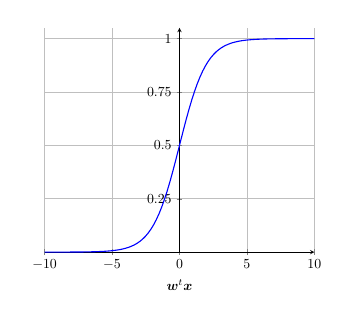
\begin{tikzpicture}[scale=0.5]
            \begin{axis}%
              [ %%%%%%%%%%%%%%%%%
              grid=major, %
              xmin=-10, % 
              xmax=10, % 
              axis x line=bottom, % 
              ytick={0,.25,.5,.75,1.0}, %
              ymax=1.05, % 
              axis y line=middle, % 
              xlabel = $\scal{\seq{w}}{\x}$, %
              %ylabel = $$, % 
              every  axis y label/.style={at={(current axis.north  west)},above=2mm} ]% 
              %%%%%%%%% binary classif in green
              \addplot%
              [ blue,thick,%
              mark=none, samples=100, domain=-10:10, ]
              (x,{1/(1+exp(-x))});
            \end{axis}
          \end{tikzpicture}
        \end{center}
        \end{minipage}
    \end{column}
  \end{columns}
\end{frame}

%%%%%%%%%%%%%%%%%%%%%%%%%%%%%%%%%%%%%%%%%%%%%%%%%%%%%%%%%%%%%%%%
\begin{frame}
  \frametitle{Logistic regression}

  The class $\class$ is the outcome of the binary random variable $\rvclass$
  \begin{block}{The sigmoid/logistic function}
    \begin{align*}
      y = P(\rvclass=1 | \x) &= \sigma(w_0 + \scal{\vct{w}}{\x}) \\
      \sigma(a)  &= \frac{e^a}{1+e^a} = \frac{1}{1+e^{-a}}\\
      a&=w_0 + \scal{\vct{w}}{\x} \in \mathbb{R}
    \end{align*}
  \end{block}
  \begin{center}
    \includegraphics[width=0.4\textwidth]{./figs/student_linear_1.pdf}
    \includegraphics[width=0.4\textwidth]{./figs/sigmoid_2d}
  \end{center}
\end{frame}

\begin{frame}{Logistic regression model for binary classification}
  \begin{itemize}
  \item The model is defined by $$ \params = (w_0 , \vct{w})$$
  \item Its output is $y = P(\rvclass=1|\x) = \sigma(w_0 + \scal{\vct{w}}{\x})$
  \item The decision rule ($\class$ inference from the model output $y$):
    \begin{align*}
      c=1 &\textrm{ if } y = P(\rvclass=1|\x) > P(\class=0|\x), &\textrm{ and } c=0 \textrm{ otherwise}\\
      c=1 &\textrm{ if } y = P(\rvclass=1|\x) > 0.5, &\textrm{ and } c=0 \textrm{ otherwise}
    \end{align*}
\end{itemize}
\begin{center}
Now let us define a criterion to \textit{learn} $\params$
\end{center}
\end{frame}





\section{Objective or loss function}



\begin{frame}
  \frametitle{Refresher:  Bernoulli distribution}
  Let $\class$ be the outcome of a binary random variable $\rvclass$
  \begin{block}{A Bernouilli distribution of parameter $\bern$}
    \begin{align*}
      P(\rvclass=1|\bern) &= \bern\\ 
      P(\rvclass=0|\bern) &= 1-\bern \\
      P(\rvclass=\class|\bern) &= \bern^{\class} (1-\bern)^{1-\class}
    \end{align*}
  \end{block}
  For  $n$ observations i.i.d  (independent, identically distributed) : $(\class\sid{1}, ... , \class\sid{n} )$
  \begin{align*}
    P((\class\sid{1}, ... , \class\sid{n} )|\bern) &= \prod_{i=1}^n P(\rvclass=\classi|\bern) = \prod_{i=1}^n \bern^{\classi} (1-\bern)^{1-\classi}\\
    \log P((\class\sid{1}, ... , \class\sid{n} )|\bern) &= \sum_{i=1}^n \log P(\rvclass=\classi|\bern) \\
    &= \sum_{i=1}^n \big[ {\classi}\log\bern + (1-\classi)\log (1-\bern) \big]
  \end{align*}
  \end{frame}

G
  
\begin{frame}
  \frametitle{The conditionnal ``Likelihood'' measured on $\dataset$}
     Given $\dataset = (\exi,\classi)_{i=1}^n = (\datax,\datac)$ and a logistic regression model, $\params =  (w_0, \vct{w})$. 
     \begin{align*}
       P(\datac | \datax, \params) &= \prod_{i=1}^n P(\rvclass = \classi| \exi, \params) \\
       P(\datac | \datax, \params) &= \prod_{i=1}^n\bern\sid{i}^{\classi} (1-\bern\sid{i})^{1-\classi}\\
       \bern\sid{i} &= y\sid{i} = \sigma(w_0 + \scal{\vct{w}}{\exi})  = \frac{1}{1+e^{-(w_0 + \scal{\vct{w}}{\exi})}}
     \end{align*}git 
     \begin{block}{The loss function (to minimize)}
       \begin{align*}
         \fullloss &= - log(P(\datac | \datax, \params) ) =  \sum_{i=1}^n  {\color{red} - \big(  \classi log(y\sid{i} )+ (1-\classi) log(1-y\sid{i})  \big)}\\
                   &= \sum_{i=1}^n  {\color{red} \ploss(\params,\exi,\classi) }, \textrm{ with } {\color{red} \ploss(\params,\exi,\classi)} \textrm{ the pointwise loss.}
       \end{align*}
     \end{block}
\end{frame}


\section{Optimization/Learning: gradient descent}
%%%%%%%%%%%%%%%%%%%%%%%%%%%%%%% SGD 
\begin{frame}{Optimisation Program}
  Let $\dataset = (\exi,\class\sid{i})_{i=1}^n = (\datax,\datac)$, and a  logistic regression model, $\params =  (w_0, \vct{w})$. \\
  \begin{block}{The loss function}
  $$
  \fullloss = - log(P(\datac | \datax, \params) ) = -
  \big(\sum_{i=1}^n \class\sid{i} log(\bern\sid{i} )+ (1-\class\sid{i}) log(1-\bern\sid{i} )
  \big)
  $$
  
  with:
  $$       \bern\sid{i} = \sigma(w_0 + \scal{\vct{w}}{\exi})  = \frac{1}{1+e^{-(w_0 + \scal{\vct{w}}{\exi})}}$$
\end{block}



\begin{block}{Learning = optimisation}
  \begin{center}
    Find $\params$ in ordre to minimize $\fullloss$ ?
  \end{center}
\end{block}
\end{frame}


\begin{frame}{Function minimization}
  \begin{block}{Bad news}
    No closed form solution in general ! 
  \end{block}
  \begin{block}{Good news}
    \begin{itemize}
    \item The function is convex \textit{w.r.t} $\params$
    \item Convex functions are ``easy'' to minimize
    \item[$\rightarrow$] An efficient, easy and generic algorirthm exists: 
      \begin{center}
        The (stochastic)  gradient descent with many variants  
      \end{center}
    \end{itemize}
  \end{block}
\end{frame}


\begin{frame}{A convex function}
  \begin{center}
    
% \shorthandoff{;} with babel french
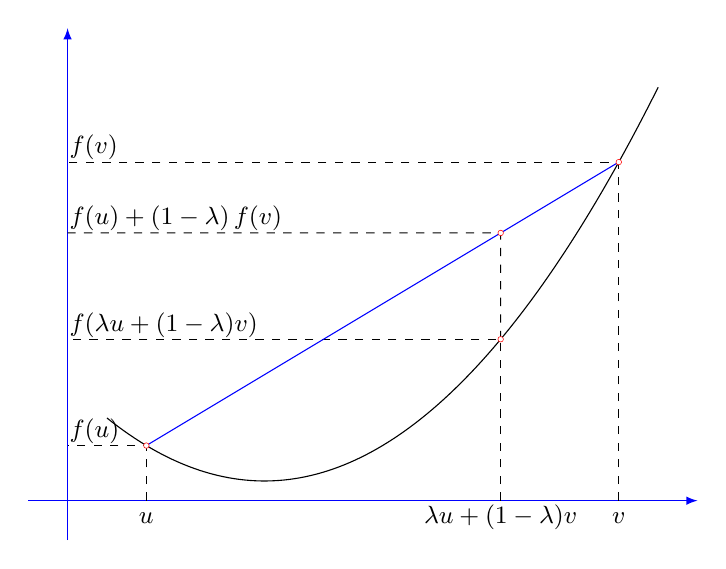
\begin{tikzpicture}[declare function={f(\x)=(\x-1)*(\x-1)/2 + 0.1;},x={(2.5cm,0)},y={(0,2.5cm)},samples=101,font=\small,inner sep=0.5pt]
  \draw[blue,-latex] (-0.2,0) -- (3.2,0);
  \draw[blue,-latex] (0,-0.2) -- (0,2.4);
  \coordinate (O) at (0,0);
  \draw plot[domain=0.2:3,variable=\x] ({\x},{f(\x)});
  \foreach [count=\Z] \X/\Y in {0.4/{u},2.2/{\lambda u +(1-\lambda) v},2.8/{v}}
  {\draw[dashed] (\X,0) coordinate (X\Z) node[below]{$\strut\Y$} -- (\X,{f(\X)}) coordinate (F\Z)
    -- (0,{f(\X)}) node[above right]{$f(\Y)$};}
  \draw[blue] (F1) -- (F3);
  \draw[dashed] (F2) --
  (intersection cs:first line={(X2)--(F2)}, second line={(F1)--(F3)})
  coordinate (F4) -- (O|-F4) node[above right]{$f(u)+(1-\lambda)\,f(v)$};
  \foreach \X in {1,...,4}
  {\draw[very thin,red,fill=white] (F\X) circle(1pt);}
\end{tikzpicture}
  
  \end{center}
$$  f\left(\lambda u +(1-\lambda)v\right)\leq \lambda\,f(u)+(1-\lambda)\,f(v).$$
\end{frame}


\begin{frame}
  \frametitle{Gradient Descent - intuition}
  How to reach the minimum ? How to recognize it ?

  % $\rightarrow$ Fonction convexe : ouf !
  %Analogie brouillard
  \begin{alertblock}{Caution :}
    \begin{itemize}
    \item The whole landscape is unknown
    \item Only pointwise knowledge: the function value and its
      (partial) derivatives
    \end{itemize}
  \end{alertblock}
  \begin{center}
    \includegraphics[width=0.5\textwidth]{./figs/brouillard.jpg}
  \end{center} 
\end{frame}


\begin{frame}{Interpretation of partial derivative}
  \begin{columns}
    \begin{column}{0.5\textwidth}
      \includegraphics[width=0.9\textwidth]{./figs/derive_1.pdf}
    \end{column}
    \begin{column}{0.5\textwidth}
      \begin{align*}
        w_k &= w_k + \eta \frac{\partial \ploss(\params,\exi,\classi) }{\partial
          w_k}\ \\
        &\ploss(\params,\exi,\classi) \nearrow
      \end{align*}
    \end{column}
  \end{columns}
  \begin{columns}
    \begin{column}{0.5\textwidth}
      \includegraphics[width=0.9\textwidth]{./figs/derive_2.pdf}
    \end{column}
    \begin{column}{0.5\textwidth}
      \begin{align*}
        w_k &= w_k - \eta \frac{\partial \ploss(\params,\exi,\classi)}{\partial
          w_k}\ \\
         &\ploss(\params,\exi,\classi) \searrow
      \end{align*}
\end{column}
  \end{columns}
  \begin{center}
\important{    $\eta > 0$ and small}
  \end{center}
\end{frame}


\begin{frame}{Minimization of  $\ploss$ \textit{w.r.t} $w_k$}

  \begin{columns}[c]
    
    \column{.5\textwidth}
    \begin{block}{Sketch}
      \setbeamertemplate{enumerate items}[default]
      \begin{enumerate} \setcounter{enumi}{-1}
      \item Start from a random point, 
      \item evaluate the slope, 
      \item follow it a bit, and \\loop back to the previous step
    \end{enumerate}
    \end{block}
    
    \column{.4\textwidth}
    \begin{center}
      \includegraphics[width=\textwidth]{./figs/velo.jpg}
    \end{center}
    
  \end{columns}

  \begin{block}{Algorithm}
    \begin{itemize}
    \item Pick $\eta>0$ and the initial value of $w_k$.
    \item while \textit{true} :
      \begin{itemize}
      \item compute $\ploss(\params,\exi,\classi)$

      \item compute the derivative and update $w_k$
$$      w_k= w_k - \eta \frac{\partial \ploss(\params,\exi,\classi) }{\partial
  w_k}
$$
\end{itemize}
\end{itemize}
\end{block}
\end{frame}

\begin{frame}{``Convergence'' }
At the minimum: 
  $$
\frac{\partial \ploss(\params,\exi,\classi) }{\partial
  w_k}  = 0
$$
\begin{center}
  \includegraphics[width=0.6\textwidth]{./figs/derive_null.pdf}
\end{center}

\end{frame}


\begin{frame}
  \frametitle{The learning rate : $\eta$}

\begin{itemize}
  \item small  steps: a valid approximation but boring ! 
  \item large steps: oscillation and divergence 
\end{itemize}
  \begin{center}
    \includegraphics[width=\textwidth]{./figs/pas.jpg}
  \end{center}

  \begin{itemize}
    \item Constant or adaptative $\eta$
    \item This is the role of the \textit{optimizer} !
  \end{itemize}
\end{frame}


\begin{frame}{Generalization : the gradient}
  \begin{itemize}
  \item All the parameters are in one vector : $\params = (w_0,\vct{w}) = (w_0,w_1,w_2,... ,w_{\nfeats})$
  \item Compute all the partial derivatives and store them in one
    vector: 
    \begin{displaymath}
              \left(
          \begin{array}{l}
            \partial{\ploss(\params,\exi,\classi)}/\partial{w_0}\\
            \partial{\ploss(\params,\exi,\classi)}/\partial{w_1}\\
            \partial{\ploss(\params,\exi,\classi)}/\partial{w_2}\\
...\\
            \partial{\ploss(\params,\exi,\classi)}/\partial{w_{\nfeats}}
            \end{array} 
          \right) = \vgrad{\params,\exi,\classi}{\ploss}
    \end{displaymath}
  \end{itemize}
  
  \begin{center}
    $\vgrad{\params}{\ploss}$ is the gradient (vector)  of $l$ w.r.t $\params$.
  \end{center}
\end{frame}

\begin{frame}{Gradient descent in 2D }
  \begin{center}
    \includegraphics[width=0.6\textwidth]{./figs/sgd}
  \end{center}
\end{frame}


\begin{frame}{Gradient descent: the algorithm}
  \framesubtitle{Batch / Online}
  \begin{block}{Batch minimization}
    while: 
        \begin{displaymath}
          \left.
            \begin{array}{ll}
              \textrm{Pour } i = 1 ... n : \\
              &\fullloss +=   \ploss(\params,\exi,\classi) \\
              &\vgrad{\params}{\fullloss} += \vgrad{\params}{  \ploss(\params,\exi,\classi)  } \\
              \params = \params - \eta  \vgrad{\params}{\fullloss}
            \end{array}\right\} \textrm{ one epoch}
        \end{displaymath}
  \end{block}

  \begin{block}{Stochastic Gradient Descent}
    while: 
        \begin{displaymath}
          \left.
            \begin{array}{ll}
              \textrm{shuffle } \dataset\\
              \textrm{for } i = 1 ... n : \\
              &\fullloss +=   \ploss(\params,\exi,\classi) \\
              &\params = \params - \eta \vgrad{\params}{\ploss(\params,\exi,\classi)  } \\
            \end{array}\right\} \textrm{ one epoch}
        \end{displaymath}
  \end{block}
  \begin{center}
    \important{A trade-off: the mini-batch}
  \end{center}
  \end{frame}

  \begin{frame}{A terminololy point}
    \begin{block}{Gradient Descent}
      A simple yet efficient algorithm to minimize a convex function
    \end{block}
    \begin{block}{Batch \textit{vs} Online}
      \begin{itemize}
      \item Batch: consider the whole $\dataset$ to estimate the gradient and the update
      \item Online: consider the training examples one by one
      \item Mini-batch: the trade-off
      \end{itemize}
    \end{block}
    \begin{block}{Stochastic}
      For online and mini-batch training: randomize the order in $\dataset$
    \end{block}
  \end{frame}


\section{Summary}
\begin{frame}
  \frametitle{Summary}
  \begin{block}{Machine Learning overview}
    \begin{itemize}
    \item A model defines a \important{function}:
      $\x \rightarrow \seq{y}$
    \item The output is then used by a decision rule.
    \item This function is defined by the parameters $\params$.
    \item \important{Training/Learning} finds the good values for
      $\params$
    \item How ? by minimizing a \important{loss function} $\fullloss$.
    \item How ? by \important{Stochastic Gradient Descent}
    \item The \important{learning rate} is an
      \important{hyper-parameter}.
    \end{itemize}
  \end{block}
  \begin{block}{From logistic regression to artificial neurone}
    \begin{itemize}
    \item An artificial neurone is a \important{linear model} followed by a
      non-linear \important{activation}
    \item With the sigmoid activation, it is similar to the
      \important{logistic regression}
    \end{itemize}
  \end{block}
\end{frame}

%%%%%%%%%%%%%%%%%%%%%%%%%%%%%%%%%%%%%%%%%%%%%%%%
\bibliographystyle{../styles/naaclhlt2012}
{\footnotesize \bibliography{./alex}}
%%%%%%%%%%%%%%%%%%%%%%%%%%%%%%%%%%%%%%%%%%%%%%%%
\end{document}
